
\subsubsection{Zakazivanje isporuka}

\begin{itemize}
	\item Kratak opis:
		\begin{itemize}
			\item Koordinator pravi raspored dostavljačima.
		\end{itemize}
	\item Učesnici:
		\begin{itemize}
		    \item Koordinator
		\end{itemize}
	\item Preduslovi:
		\begin{itemize}
		    \item Postoji bar jedan dostupan dostavljač.
		    \item Sistem je u funkciji.
		\end{itemize}
	\item Postuslovi:
		\begin{itemize}
			\item Svaka narudžbina je dodeljena nekom od dostavljača.
	\end{itemize}
	\item Osnovni tok:
		\begin{enumerate}
            \item Koordinator pristupa sistemu i prolazi kroz sve narudžbine koje bi trebalo da se obave sledeće nedelje.
            \item Sistem pristupa bazi podataka i generiše listu svih zakazanih narudžbina za sledeću nedelju.
            \item Koordinator selektuje jednu od narudžbina.
            \item Sistem pristupa bazi podataka i generiše listu dostavljača koji su slobodni u zakazano vreme dostave selektovane narudžbine.
           \item Koordinator narudžbini dodeljuje dostavljača.
           \item Sistem narudžbini ažurira dodeljenog dostavljača.
            \item Sistem klijentu šalje automatski mejl kojim ga obaveštava da je porudžbina obrađena i podseća  ga u koje vreme mora da bude kod kuće da bi primio porudžbinu.
            \item Koordinator dostavljačima preko sistema prosleđuje njegovu listu isporuka za narednu nedelju.
		\end{enumerate}
	  \textit{Koraci 3-7 se ponavljaju dok postoje narudžbine koje nisu dodeljene nijednom dostavljaču.}
   \item Dodatne informacije:
        \begin{itemize}
           \item Lista slobodnih dostavljača je sortirana prema razdaljini izmedju njihove izabrane regije dostave i regije u kojoj je potrebno izvršiti dostavu.
            \item Lista isporuka se sastoji od infomacija o dostavi: ime, prezime, adresa, zakazano vreme dostave i id narudžbine. 
        \end{itemize}
\end{itemize}

\begin{figure}[H]
\begin{center}
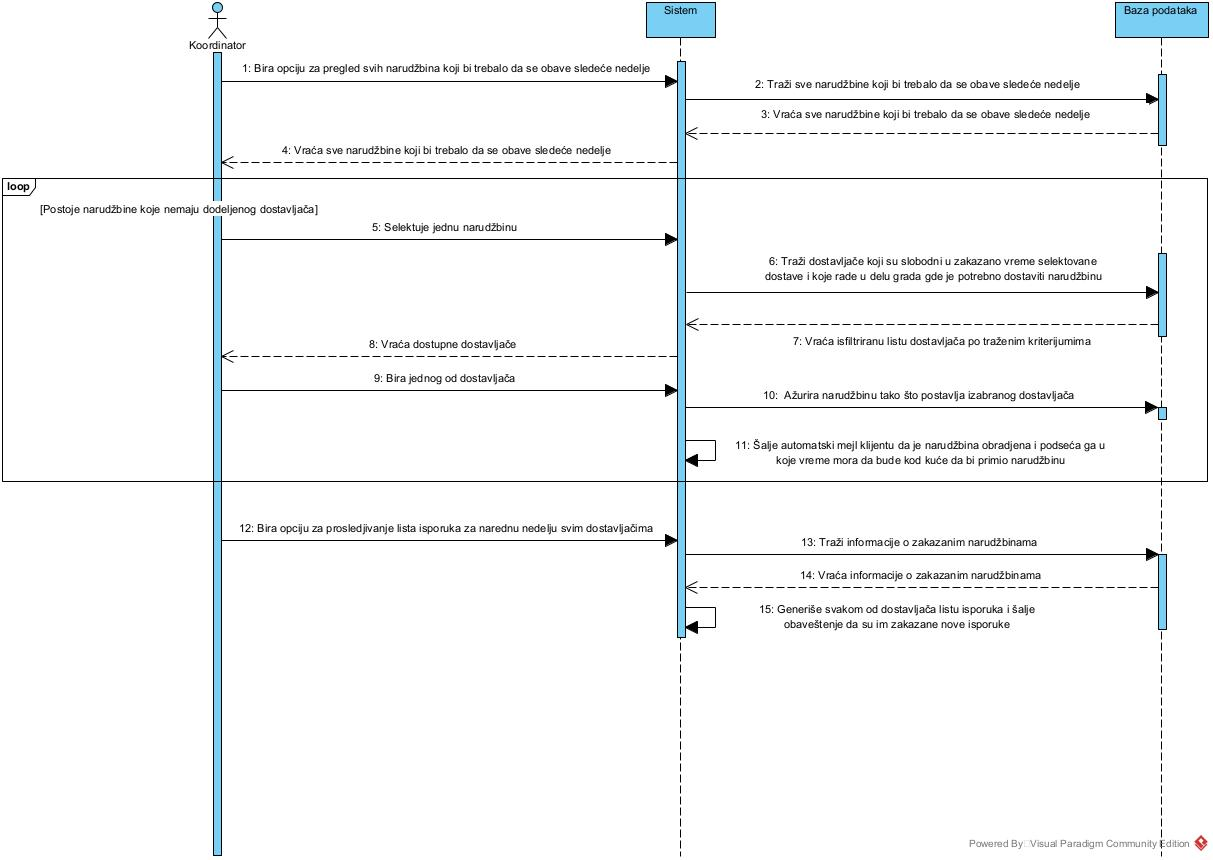
\includegraphics[width=\textwidth]{Pictures/sequence_scheduling_deliveries.jpg}
\end{center}
    \caption{Dijagram sekvenci - Zakazivanje isporuka}
\label{fig:Sequence_diagram_scheduling_deliveries}
\end{figure}

